% piracy-msc-ai.tex
% Generated from: "# Piracy — Notes for PPT (MSc AI).txt"
% Skill: docs-latex  |  Theme: Catppuccin Mocha  |  Class: beamer (16:9)

\documentclass[aspectratio=169,11pt]{beamer}

% ---------- Encoding & fonts ----------
\usepackage[utf8]{inputenc}
\usepackage[T1]{fontenc}
\usepackage{lmodern}

% ---------- Catppuccin Mocha palette ----------
\usepackage{xcolor}
\definecolor{ctpBase}{HTML}{1E1E2E}
\definecolor{ctpMantle}{HTML}{181825}
\definecolor{ctpCrust}{HTML}{11111B}
\definecolor{ctpSurface0}{HTML}{313244}
\definecolor{ctpSurface1}{HTML}{45475A}
\definecolor{ctpSurface2}{HTML}{585B70}
\definecolor{ctpOverlay0}{HTML}{6C7086}
\definecolor{ctpOverlay1}{HTML}{7F849C}
\definecolor{ctpText}{HTML}{CDD6F4}
\definecolor{ctpSubtext}{HTML}{A6ADC8}
\definecolor{ctpMauve}{HTML}{CBA6F7}
\definecolor{ctpPink}{HTML}{F5C2E7}
\definecolor{ctpRed}{HTML}{F38BA8}
\definecolor{ctpMaroon}{HTML}{EBA0AC}
\definecolor{ctpPeach}{HTML}{FAB387}
\definecolor{ctpYellow}{HTML}{F9E2AF}
\definecolor{ctpGreen}{HTML}{A6E3A1}
\definecolor{ctpTeal}{HTML}{94E2D5}
\definecolor{ctpSky}{HTML}{89DCEB}
\definecolor{ctpBlue}{HTML}{89B4FA}
\definecolor{ctpLavender}{HTML}{B4BEFE}

% ---------- Beamer theme ----------
\usetheme{default}
\usefonttheme{professionalfonts}
\setbeamertemplate{navigation symbols}{}

\setbeamercolor{normal text}{fg=ctpText,bg=ctpBase}
\setbeamercolor{structure}{fg=ctpMauve}
\setbeamercolor{frametitle}{fg=ctpMauve,bg=ctpBase}
\setbeamercolor{title}{fg=ctpPink}
\setbeamercolor{subtitle}{fg=ctpSubtext}
\setbeamercolor{itemize item}{fg=ctpMauve}
\setbeamercolor{itemize subitem}{fg=ctpBlue}
\setbeamercolor{enumerate item}{fg=ctpMauve}
\setbeamercolor{block title}{bg=ctpSurface0,fg=ctpMauve}
\setbeamercolor{block body}{bg=ctpMantle,fg=ctpText}
\setbeamercolor{footline}{fg=ctpSubtext,bg=ctpCrust}
\setbeamercolor{alerted text}{fg=ctpPink}
\setbeamertemplate{blocks}[rounded][shadow=false]

\setbeamerfont{frametitle}{size=\Large,series=\bfseries}
\setbeamertemplate{frametitle}{%
	\vspace{0.35cm}%
	\usebeamercolor[fg]{frametitle}\insertframetitle\par%
	\vspace{0.05cm}%
	\textcolor{ctpSurface2}{\rule{\linewidth}{0.6pt}}%
	\vspace{0.15cm}%
}

\setbeamertemplate{footline}{%
	\leavevmode%
	\hbox{%
		\begin{beamercolorbox}[wd=.72\paperwidth,ht=2.4ex,dp=1.1ex,leftskip=.3cm]{footline}%
			\usebeamerfont{footline}\insertshorttitle
		\end{beamercolorbox}%
		\begin{beamercolorbox}[wd=.28\paperwidth,ht=2.4ex,dp=1.1ex,rightskip=.3cm plus1fil]{footline}%
			\usebeamerfont{footline}\hfill\insertframenumber\,/\,\inserttotalframenumber
	\end{beamercolorbox}}%
	\vskip0pt%
}

% ---------- Packages ----------
\usepackage{booktabs}
\usepackage{tabularx}
\usepackage{colortbl}
\usepackage{fontawesome5}
\usepackage{amssymb}
\usepackage{tikz}
\usepackage{pgfplots}
\pgfplotsset{compat=1.18}
\usetikzlibrary{shapes,arrows.meta,positioning,calc,patterns}
\usepackage[most]{tcolorbox}

% ---------- Callout boxes (Catppuccin, semantic mapping preserved) ----------
\newtcolorbox{infobox}[1][]{
	colback=ctpMantle, colframe=ctpBlue, coltext=ctpText, coltitle=ctpBase,
	fonttitle=\bfseries, title={\faInfoCircle\ Info}, #1}
\newtcolorbox{warningbox}[1][]{
	colback=ctpMantle, colframe=ctpYellow, coltext=ctpText, coltitle=ctpBase,
	fonttitle=\bfseries, title={\faExclamationTriangle\ Key Point}, #1}
\newtcolorbox{dangerbox}[1][]{
	colback=ctpMantle, colframe=ctpRed, coltext=ctpText, coltitle=ctpBase,
	fonttitle=\bfseries, title={\faBolt\ Case Study}, #1}
\newtcolorbox{successbox}[1][]{
	colback=ctpMantle, colframe=ctpGreen, coltext=ctpText, coltitle=ctpBase,
	fonttitle=\bfseries, title={\faCheckCircle\ Takeaway}, #1}
\newtcolorbox{quotebox}[1][]{
	colback=ctpCrust, colframe=ctpPink, coltext=ctpText,
	fonttitle=\bfseries, #1}

% ---------- Table styling ----------
\renewcommand{\arraystretch}{1.22}
\arrayrulecolor{ctpSurface2}

% ---------- Metadata ----------
\title[Piracy in the Digital Age]{Piracy}
\subtitle{Copyright, Ownership \& the AI Frontier}
\author{MSc Artificial Intelligence}
\date{\today}

\begin{document}
	
	% ============================================================
	% 1. Title
	% ============================================================
	\begin{frame}[plain]
		\centering
		\vspace{1.4cm}
		{\usebeamercolor[fg]{title}\Huge\bfseries Piracy}\\[0.35cm]
		{\usebeamercolor[fg]{subtitle}\Large Copyright, Ownership \& the AI Frontier}\\[0.9cm]
		\textcolor{ctpSurface2}{\rule{5cm}{0.6pt}}\\[0.6cm]
		{\color{ctpSubtext}\large MSc Artificial Intelligence --- Seminar}\\[0.25cm]
		{\color{ctpOverlay0}\small \today}
	\end{frame}
	
	% ============================================================
	% 2. Definition & Scope
	% ============================================================
	\begin{frame}{Definition \& Scope}
		\begin{columns}[T,onlytextwidth]
			\begin{column}{0.52\textwidth}
				\textbf{\color{ctpMauve}Piracy / Copyright Infringement}\\[0.2cm]
				Unauthorized reproduction, distribution, or use of copyrighted material in a manner that violates the owner's \alert{exclusive rights}.\\[0.4cm]
				\begin{infobox}
					With digital technology, modern piracy produces \textbf{exact and perfect copies} --- either from hard copies or downloaded over the Internet.
				\end{infobox}
			\end{column}
			\begin{column}{0.46\textwidth}
				\textbf{\color{ctpMauve}Common forms}\\[0.2cm]
				\begin{itemize}\itemsep0.35em
					\item[\faTv] Illegal streaming sites\\
					{\footnotesize\color{ctpOverlay1}now dominant --- $\sim$96\% of TV piracy}
					\item[\faShareAlt] P2P / torrent networks\\
					{\footnotesize\color{ctpOverlay1}still active, ages 15--24}
					\item[\faCloudDownloadAlt] Cyber-lockers \& direct downloads
					\item[\faRobot] Unauthorized AI training-data scraping\\
					{\footnotesize\color{ctpOverlay1}emerging category}
				\end{itemize}
			\end{column}
		\end{columns}
	\end{frame}
	
	% ============================================================
	% 3. The Quote
	% ============================================================
	\begin{frame}{}
		\centering
		\vfill
		{\Huge\color{ctpOverlay0}\faQuoteLeft}\\[0.35cm]
		{\LARGE\itshape\color{ctpPink} If buying isn't owning,\\[0.15cm] piracy isn't stealing.}\\[0.35cm]
		{\Huge\color{ctpOverlay0}\faQuoteRight}\\[0.7cm]
		\textcolor{ctpSubtext}{\small Viral slogan, recurring across online forums}
		\vfill
	\end{frame}
	
	% ============================================================
	% 4. Sony PlayStation 2026
	% ============================================================
	\begin{frame}{The Triggering Event: Sony PlayStation (2026)}
		\begin{dangerbox}
			Sony announced that \textbf{over 550 movies} purchased by PlayStation customers would be \textbf{removed from their accounts} --- with \textbf{no refunds} and \textbf{no offline download}. Reason cited: \emph{``content licensing arrangements''} (Studio Canal).
		\end{dangerbox}
		\vspace{0.3cm}
		\centering
		
\begin{tikzpicture}[
			node distance=2.0cm,
			box/.style={rectangle, rounded corners=4pt, draw=ctpSurface2, fill=ctpSurface0,
				text=ctpText, minimum width=2.9cm, minimum height=1.1cm,
				align=center, font=\small},
			arrow/.style={-{Latex[length=2.5mm]}, thick, ctpPink}
			]
			\node[box] (buy) {\textbf{Buy button}\\ {\footnotesize next to ``Rent''}};
			\node[box, right=of buy] (own) {\textbf{``Purchased''}\\ {\footnotesize Sony's own wording}};
			\node[box, right=of own, draw=ctpRed] (gone) {\textbf{Removed}\\ {\footnotesize no refund}};
			\draw[arrow] (buy) -- (own);
			\draw[arrow] (own) -- (gone);
		\end{tikzpicture}
		\vspace{0.35cm}
		\begin{quotebox}
			\small When the distinction between \textbf{buy} and \textbf{rent} collapses, the ``theft'' framing becomes incoherent --- and the moral argument for piracy strengthens in consumers' minds.
		\end{quotebox}
	\end{frame}
	
	% ============================================================
	% 5. Gabe Newell
	% ============================================================
	\begin{frame}{Gabe Newell (Valve Co-founder, 2011)}
		\vspace{0.3cm}
		\begin{quotebox}
			\centering\large\itshape\color{ctpPink}
			``Piracy is not a pricing issue.\\[0.1cm] It's a service issue.''
		\end{quotebox}
		\vspace{0.5cm}
		\begin{itemize}\itemsep0.6em
			\item Best anti-piracy strategy is \textbf{not DRM} --- it is \textbf{better service}.
			\item \emph{``The easiest way to stop piracy is not by putting antipiracy technology to work. It's by giving those people a service that's better than what they're receiving from the pirates.''}
		\end{itemize}
		\vspace{0.3cm}
		\begin{successbox}
			Sony's 2026 action is a case study in what happens when the \textbf{service is fundamentally broken}: if ``buying'' only grants access for an undetermined time dependent on volatile licensing deals, \textbf{piracy becomes the rational alternative}.
		\end{successbox}
	\end{frame}
	
	% ============================================================
	% 6. Subscription economy
	% ============================================================
	\begin{frame}{Subscription Economy \& ``You Will Own Nothing''}
		\vspace{0.1cm}
		{\small The WEF essay popularised \textbf{``You will own nothing and be happy''} --- originally a speculative thought experiment about \textbf{access-based consumption} (capex $\rightarrow$ opex). It has since become a lightning rod for criticism of subscription models.}
		\vspace{0.35cm}
		\centering
		\begin{tabular}{@{}l l@{}}
			\toprule
			\textbf{\color{ctpMauve}Domain} & \textbf{\color{ctpMauve}Shift} \\
			\midrule
			Music      & Ownership $\rightarrow$ streaming access (Spotify, Apple Music) \\
			Video      & DVD/Blu-ray $\rightarrow$ platform subscriptions (Netflix, Disney+) \\
			Software   & Perpetual licences $\rightarrow$ SaaS subscriptions \\
			Gaming     & Physical/digital purchase $\rightarrow$ Game Pass, cloud streaming \\
			Cars       & Ownership $\rightarrow$ leasing / subscription features \\
			\bottomrule
		\end{tabular}
		\vspace{0.35cm}
		\begin{warningbox}
			\small If the \textbf{legal} market only offers \textbf{temporary, revocable access} --- often across \textbf{fragmented platforms} --- the moral distinction between ``legal access'' and ``pirated access'' narrows. Both are, functionally, \textbf{access without ownership}.
		\end{warningbox}
	\end{frame}
	
	% ============================================================
	% 7. Legal landscape
	% ============================================================
	\begin{frame}{Legal Landscape --- Traditional Cases}
		\begin{itemize}\itemsep0.8em
			\item \textbf{\color{ctpBlue}The Pirate Bay} {\footnotesize\color{ctpOverlay1}(Netherlands, 2012)}\\
			District Court of The Hague ruled that subscribers of XS4ALL and Ziggo committed copyright infringement by uploading protected works.
			\item \textbf{\color{ctpBlue}Cox Communications} {\footnotesize\color{ctpOverlay1}(US)}\\
			A Virginia jury awarded \textbf{\$1 billion} for contributory infringement. The Supreme Court later vacated the verdict --- ISPs generally \emph{not} liable for users' piracy.
			\item \textbf{\color{ctpBlue}Mulholland Drive} {\footnotesize\color{ctpOverlay1}(France)}\\
			A court ordered DVD vendors to remove copy protection, ruling it violated privacy rights when a consumer tried to transfer the film for personal use.
		\end{itemize}
		\vspace{0.4cm}
		\begin{infobox}
			\small Pattern: courts consistently distinguish between \textbf{facilitating} infringement and \textbf{committing} it --- a distinction that returns sharply in the AI cases.
		\end{infobox}
	\end{frame}
	
	% ============================================================
	% 8. AI training data piracy
	% ============================================================
	\begin{frame}{AI Training Data Piracy --- The Emerging Frontier}
		\begin{dangerbox}
			\textbf{Anthropic / Authors Guild Settlement (2026)}\\[0.2cm]
			Downloaded \textbf{hundreds of thousands of books} from LibGen and other shadow libraries to train Claude.\\[0.15cm]
			\textbf{\$1.5 billion settlement} --- the largest generative AI copyright settlement in US history. Covers $\sim$480{,}000 works; over 90\% of rights holders filed claims.
		\end{dangerbox}
		\vspace{0.3cm}
		\begin{warningbox}
			\textbf{Sony \& Warner Music v.\ Anthropic (2026)}\\[0.2cm]
			Trained Claude on \textbf{tens of thousands} of copyrighted compositions via \textbf{pirated downloads and scraping}. Seeking up to \textbf{\$150{,}000 per willful infringement} --- potential liability in the billions.\\
			{\footnotesize\color{ctpOverlay1}\emph{``Even the most revolutionary technology must develop within the law.''}}
		\end{warningbox}
	\end{frame}
	
	% ============================================================
	% 9. AI paradox / implication
	% ============================================================
	\begin{frame}{The AI Paradox --- Why This Matters for MSc AI}
		\vspace{0.2cm}
		\begin{columns}[T,onlytextwidth]
			\begin{column}{0.48\textwidth}
				\textbf{\color{ctpMauve}What the cases establish}\\[0.25cm]
				\begin{itemize}\itemsep0.5em
					\item Training AI on copyrighted works is \textbf{not inherently illegal}.
					\item \textbf{Acquiring them through piracy is.}
					\item \textbf{Data provenance matters legally.} Scraping or downloading pirated data is a distinct, actionable infringement --- even if training itself is later deemed fair use.
				\end{itemize}
			\end{column}
			\begin{column}{0.48\textwidth}
				\textbf{\color{ctpMauve}Where it's heading}\\[0.25cm]
				\begin{itemize}\itemsep0.5em
					\item \$1.5B was \emph{``clearly not enough to deter''} a company valued at \textbf{\$2 trillion} --- the settlement is priced as a \textbf{cost of doing business}.
					\item A \textbf{market-based solution is emerging}: AI companies signing licensing deals with publishers (OpenAI, Anthropic).
				\end{itemize}
			\end{column}
		\end{columns}
		\vspace{0.4cm}
		\begin{quotebox}
			\centering\small\itshape\color{ctpPink}
			AI companies trained on pirated data to build tools that could displace the very creators whose work was pirated.
		\end{quotebox}
	\end{frame}
	
	% ============================================================
	% 10. Statistics
	% ============================================================
	\begin{frame}{Statistics --- The Piracy Resurgence}
		\begin{columns}[T,onlytextwidth]
			\begin{column}{0.52\textwidth}
				\centering
				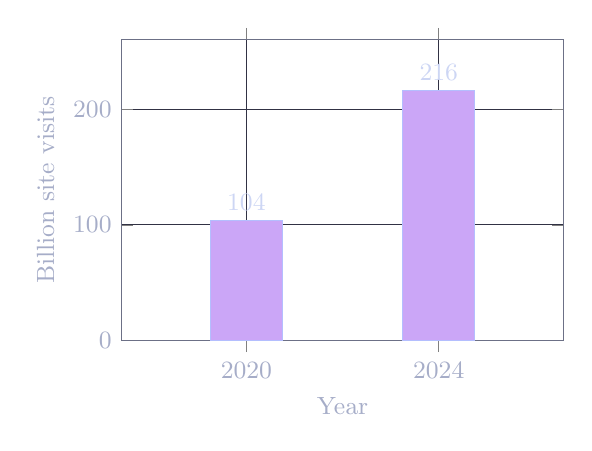
\begin{tikzpicture}
					\begin{axis}[
						ybar, bar width=26pt,
						width=7.2cm, height=5.4cm,
						axis line style={ctpOverlay0},
						every axis label/.style={color=ctpSubtext,font=\small},
						tick label style={color=ctpSubtext,font=\small},
						xlabel={Year}, ylabel={Billion site visits},
						symbolic x coords={2020,2024},
						xtick=data,
						nodes near coords,
						nodes near coords style={color=ctpText,font=\small\bfseries},
						ymin=0, ymax=260,
						enlarge x limits=0.65,
						grid=major,
						grid style={ctpSurface0, line width=0.3pt},
						]
						\addplot[fill=ctpMauve, draw=ctpLavender] coordinates {(2020,104) (2024,216)};
					\end{axis}
				\end{tikzpicture}\\[0.1cm]
				{\small\color{ctpPink}\textbf{+66\%} in four years}
			\end{column}
			\begin{column}{0.46\textwidth}
				\vspace{0.15cm}
				\centering
				\begin{tabular}{@{}l r@{}}
					\toprule
					\textbf{\color{ctpMauve}Metric} & \textbf{\color{ctpMauve}Figure} \\
					\midrule
					Pirated video visits (2023) & 229\,B/yr \\
					Monthly infringing visits & $\sim$7\,B \\
					Subscription fatigue & 62\% \\
					Manga piracy growth & +56\% \\
					TV piracy from streaming & 96\% \\
					Sweden 15--24 admitting & 25\% \\
					\bottomrule
				\end{tabular}
				\vspace{0.3cm}
				\begin{infobox}
					\small \textbf{Driver:} ``streaming fatigue'' --- rising prices, ad tiers, password crackdowns, fragmentation. Consumers \textbf{mix paid subscriptions with piracy}, choosing on convenience.
				\end{infobox}
			\end{column}
		\end{columns}
	\end{frame}
	
	% ============================================================
	% 11. Discussion
	% ============================================================
	\begin{frame}{Discussion Points}
		\small
		\begin{enumerate}\itemsep0.55em
			\item \textbf{Is ``piracy isn't theft'' coherent?} If the legal transaction is a licence, not a sale, what exactly is stolen --- the licence? potential revenue? the exclusive distribution right?
			\item \textbf{Service vs.\ price.} Piracy fell during streaming's golden era (2015--2020) and rose as service quality declined. Is piracy primarily a \textbf{market failure}, not a moral failure?
			\item \textbf{The AI paradox.} The \$1.5B Anthropic settlement is both a deterrent and a \textbf{cost of doing business} for a \$2T company.
			\item \textbf{Digital ownership regulation.} California's \textbf{AB 2426} requires platforms to disclose licence-not-ownership. EU \textbf{Digital Fairness} / \textbf{DSA} push similarly. Regulation --- or just better-disclosed ``you own nothing''?
			\item \textbf{Preservation.} Piracy is often the \emph{only} way media survives delisting, as Sony's 550-movie removal shows. Is there a \textbf{public-interest justification}?
		\end{enumerate}
	\end{frame}
	
	% ============================================================
	% 12. Conclusion
	% ============================================================
	\begin{frame}{}
		\centering
		\vfill
		{\LARGE\color{ctpMauve}\bfseries Piracy is a symptom, not a cause.}\\[0.8cm]
		{\color{ctpSubtext}\large It rises where ownership is revoked,\\
			access is fragmented, and service is broken.}\\[1.0cm]
		\textcolor{ctpSurface2}{\rule{5cm}{0.6pt}}\\[0.6cm]
		{\color{ctpOverlay0}\small MSc Artificial Intelligence --- Seminar}
		\vfill
	\end{frame}
	
\end{document}